\documentclass[12pt,a4paper]{article}
%============================================================
% Pakete
%============================================================
\usepackage[utf8]{inputenc}
\usepackage[german]{babel}
\usepackage[T1]{fontenc}
\usepackage{amsmath}
\usepackage{amsfonts}
\usepackage{amssymb}
\usepackage{makeidx}
\usepackage{graphicx}
\usepackage[left=2cm,right=2cm,top=2cm,bottom=2cm]{geometry}
\usepackage{tikz}
\usepackage{pdfpages}
\pagestyle{plain}
\usepackage{bm}
\usepackage{ulem}
\usepackage{url}

%Kopf und Fußzeile:
\usepackage{fancyhdr}
\pagestyle{fancy}
\fancyhf{} %alles löschen
%Fußzeile:
%\fancyfoot[C]{\thepage}
%Kopfzeile:
%\fancyhead[R]{\chapter}
%\renewcommand{\headrulewidth}{0.4pt}
\renewcommand{\footrulewidth}{0.4pt}
\usepackage{array}   % for \newcolumntype macro
\newcolumntype{C}{>{$}c<{$}} % math-mode version of "c" column type

\fancyhead[L]{P22.a Wissenschaftliches Rechnen -- CP II}
%\fancyhead[C]{Dr. Bj\"orn Leder}
\fancyhead[R]{Abgabe Projekt 4}
\fancyfoot[L]{\today}
\fancyfoot[R]{Seite \thepage}
\fancyfoot[C]{Benjamin Dummer}

\DeclareMathOperator{\TR}{Tr}

% Code-Listings
\usepackage{listings}
\lstset{
  language=Python,
  showstringspaces=false}

% Ganze Dateien als Verbatim einbinden
%\usepackage{verbatimfiles} % downloaded from ctan.org
%============================================================
% Titel, Autor, Datum
%============================================================
\title{P22.a Wissenschaftliches Rechnen -- CP II}
\author{Benjamin Dummer}
\date{\today}

%============================================================
% Dokument
%============================================================
\begin{document}

% Titel erstellen
%\maketitle


\lstset{numbers=left}
% Matlab-Datei einbinden

\begin{center}
\large{\textbf{CP II -- Projekt 4: Neuronale Netze} \\
~\\
\small{-- Benjamin Dummer (532716) --}\\
~\\
Datum: \today}
\end{center}
\hrule 

\section*{Aufgabe 4.1: Hopfield-Modell mit asynchronem und synchronem Update}
\subsection*{Aufgabenstellung:}
Das Hopfield-Modell soll, wie in der Literatur (\cite{skript}, \cite{buch}) beschrieben, mit asynchronem und synchronem Update realisiert werden. Das Netzwerk soll für verschiedene Anzahlen gespeicherter Bilder untersucht werden.
\subsection*{Lösung:}
Die Umsetzung ist in dem Python-Skripten \url{task_4-1.py} \& \url{task_4-1_big-run.py} und der dazugehörigen Funktionenbibliothek \url{hopfield_func.py} zu finden. Als Standard-Parameter werden in der gesamten Bearbeitung folgende Werte verwendet:
\begin{itemize}
    \item Anzahl Neuronen: $N = 100$
    \item Anzahl gespeicherter Bilder: $P \in \{10, 20, 30\}$
\end{itemize}
Anhand verschiedener Testläufe für die Konvergenz mit synchronem und asynchronem Update wird die maximale Iterationszahl auf $100$ festgelegt, da eine Konvergenz, wenn sie eintritt, deutlich schneller erreicht ist.

Die folgende Tabelle zeigt die gemittelten Ergebnisse für die relativen Fehler (Hamming-Abstände) nach einer Iteration $\delta_1$ und nach der Konvergenz $\delta_{\inf}$ sowie die Anzahl Iterationen bis zur Konvergenz $N_{\inf}$ für die verschiedenen Anzahlen gespeicherter Bilder bei asynchronem Update:
\begin{center}
\begin{tabular}{C|C|C|C}
	P & \delta_1 [\%] & \delta_{\inf} [\%] & N_{\inf} \\ \hline
	10 & 0.07 & 0.2 & 1.1 \\
	20 & 1.8 & 7 & 3.0 \\
	30 & 5.4 & 21 & 5.8
\end{tabular}
\end{center}
Die einzelnen Werte sind ohne Fehlerangaben, da es keine explizite Fehleranalyse gab. Hier wurden jeweils $100$ verschiedene Bilderkonfigurationen gemittelt. Durch verschiedene Testläufe zeigte sich, dass insbesondere für $P=10$ der relative Fehler der einzelnen Werte durchaus bei $50\%$ liegen kann. Trotzdem lässt sich eindeutig ein Trend erkennen. Schaut man sich zusätzlich nicht gemittelte Datensätze genauer an, ist eindeutig zu erkennen, dass für $P=10$ nur sehr selten eine Veränderung des Netzwerks auftritt. Eine Iteration bedeutet im Zusammenhang mit dem Abbruchkriterium, dass das Netzwerk vor und nach der Iteration exakt den gleichen Zustand hat.

Für den Fall des synchronen Updates fällt auf, dass die Fehler und die Konvergenzgeschwindigkeit (wenn eine Konvergenz eintritt) grundsätzlich ähnlich bleiben. Jedoch tritt nicht immer eine Konvergenz ein und der Anteil der nicht konvergierenden Versuche steigt mit der Anzahl der gespeicherten Bilder.

\section*{Aufgabe 4.2: Konvergenz und endliche Temperatur}
\subsection*{Aufgabenstellung:}
Für das Hopfield-Modell mit asynchronem Update soll das Konvergenzverhalten zu gespeicherten Bildern untersucht werden und eine endliche Temperatur implementiert werden.
\subsection*{Lösung:}
Die Umsetzung ist in dem Python-Skripten \url{task_4-2.py} \& \url{task_4-2_big-run.py} und der dazugehörigen Funktionenbibliothek \url{hopfield_func.py} zu finden. Es wurden die in Aufgabe 4.1 benannten Parameter weiter genutzt. Zusätzlich wurde die Fehlertoleranz für eine Konvergenz auf $5\%$ festgelegt.

Bei Testläufen mit der vorgeschlagenen Anzahl von zufälligen Start-Konfigurationen wurde festgestellt, dass die Ergebnisse sehr stark streuen und es somit eine starke Abhängigkeit des Konvergenzverhaltens von dem Set gespeicherter Bilder vs. Startkonfiguration gibt.
Außerdem war schnell zu erkennen, dass für $P \in \{20, 30\}$ überwiegend spurious states erreicht werden und es nur sehr wenig "`Wiedererkennung"' im Netzwerk gibt. Dies deckt sich mit der Erwartung, dass ein Hopfield-Netzwerks nur mit $P < 0.138 N$ einen nützlichen Speicher darstellt (Stichwort: Kapazität, \cite{buch}). Um genauere Aussagen über den Anteil von spurious states zu erhalten, muss die Statistik für die Simulation erhöht werden. Genauso kann auf den zweiten Teil der Frage, ob bei der Implementation von endlicher Temperatur ein $\beta$ existiert, für dass sich der Anteil der spurious states verringert, nur mit größerer Statistik eingegangen werden. Für die Plots in Abb. \ref{P10} wurden jeweils $1000$ zufällige Startkonfigurationen für $1000$ verschiedene Sets gespeicherter Bilder simuliert. Dabei wurden unterschiedliche "`Dauern"' der endlichen Temperatur untersucht. Der Anteil der spurious states für das Netzwerk ohne endliche Temperatur ist jeweils durch die gestrichelte, schwarze Linie dargestellt. Auch für diese Ergebnisse wurde keine aufwändige Fehleruntersuchung durchgeführt, jedoch erlaubt der Verlauf der Kurven einen qualitativen Eindruck über die Schwankungen der gemessenen Werte.

Zunächst muss festgestellt werden, dass in Abb. \ref{P10} \textit{Oben} die Kurve für 100 Iterationen mit endlicher Temperatur fehlerhaft ist, da vergessen wurde, das Konvergenzlimit zu verändern. Trotzdem liegen die Werte für $\beta > 4$ vermutlich nah an den tatsächlichen, da sich die Zustände bei ausreichend kleinem Rauschen nach so vielen Iterationen sehr nah am Minimum im Zustandsraum befinden. Leider blieb keine Zeit, um noch eine Simulation für eine Korrektur der Werte anzustoßen.

Insgesamt ist für Abb. \ref{P10} \textit{Oben} und \textit{Mitte} (für letztere nur in gewissem Rahmen) zu erkennen, dass die Dauer der endlichen Temperatur einen deutlichen Einfluss auf die Ergebnisse hat. So tritt das Minimum in der Kurve erst für eine ausreichend lange Dauer sichtbar auf. Es zeigt sich auch, dass ein starkes Rauschen (kleines $\beta$) zu einer Erhöhung des Anteils der spurious states führt (im Vergleich zum System ohne endliche Temperatur). Außerdem nähern sich die Kurven, wie zu erwarten, für $\beta \rightarrow \inf$ dem Wert für das System ohne endliche Temperatur an. Für Abb. \ref{P10} \textit{Unten} hat keiner der Parameter einen Einfluss auf das Ergebnis.

Für $P = 10$ existiert also ein $\beta_{min}$ für das der Anteil der spurious states gesenkt wird mit ungefähr $4 < \beta_{min} < 9$. Für diese Anzahl gespeicherter Bilder ist ein Optimum von $30 - 40 \%$ für den Anteil von spurious states zu erwarten.

Auch für $P = 20$ existiert ein solches $\beta_{min}$ mit ungefähr $5 < \beta_{min} < 18$. Dazu sollte allerdings festgestellt werden, dass die Daten für $P=20$ eine recht geringe Aussagekraft haben, da es sich um minimale Änderungen handelt.

\begin{figure}[p]
\centering
    \vspace{-0.5cm}
    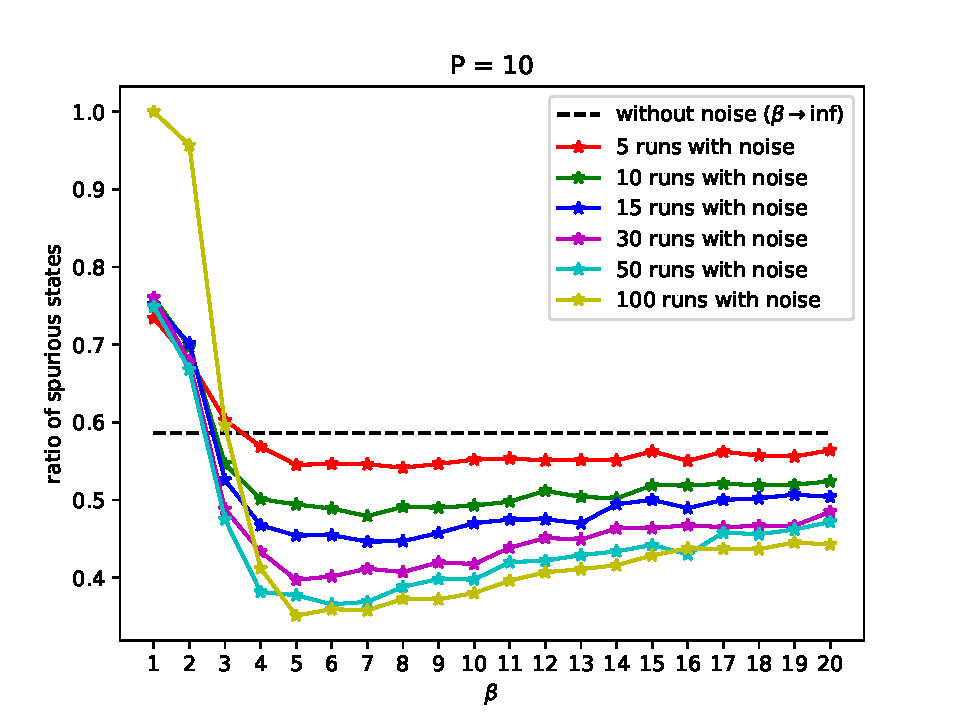
\includegraphics[width=0.63\textwidth]{../pics/fig_P10_w-noise.pdf}
    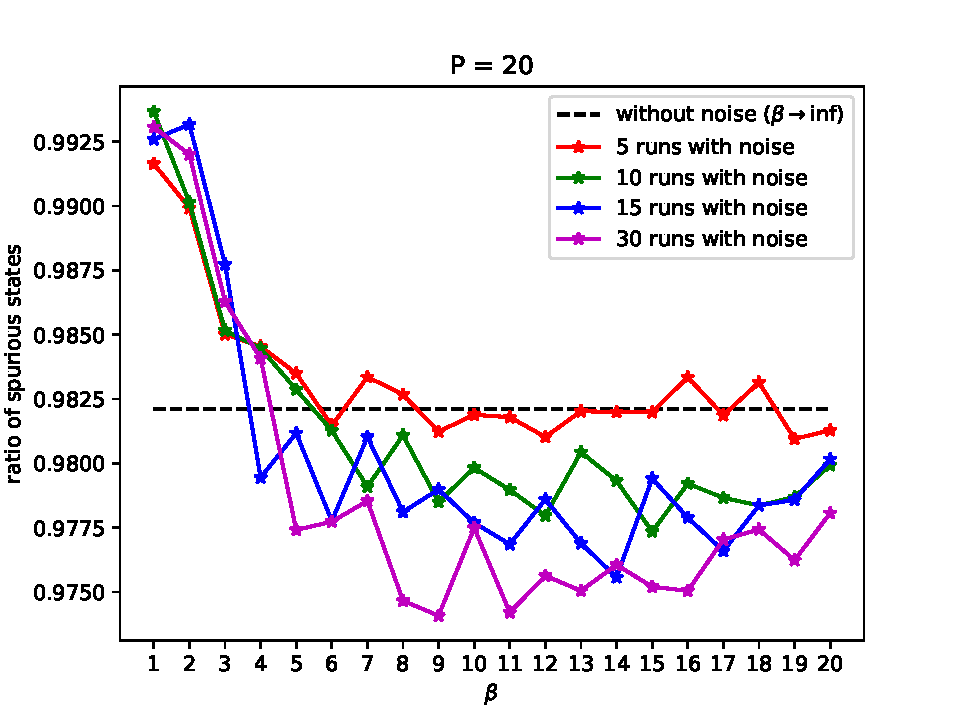
\includegraphics[width=0.63\textwidth]{../pics/fig_P20_w-noise.pdf}
    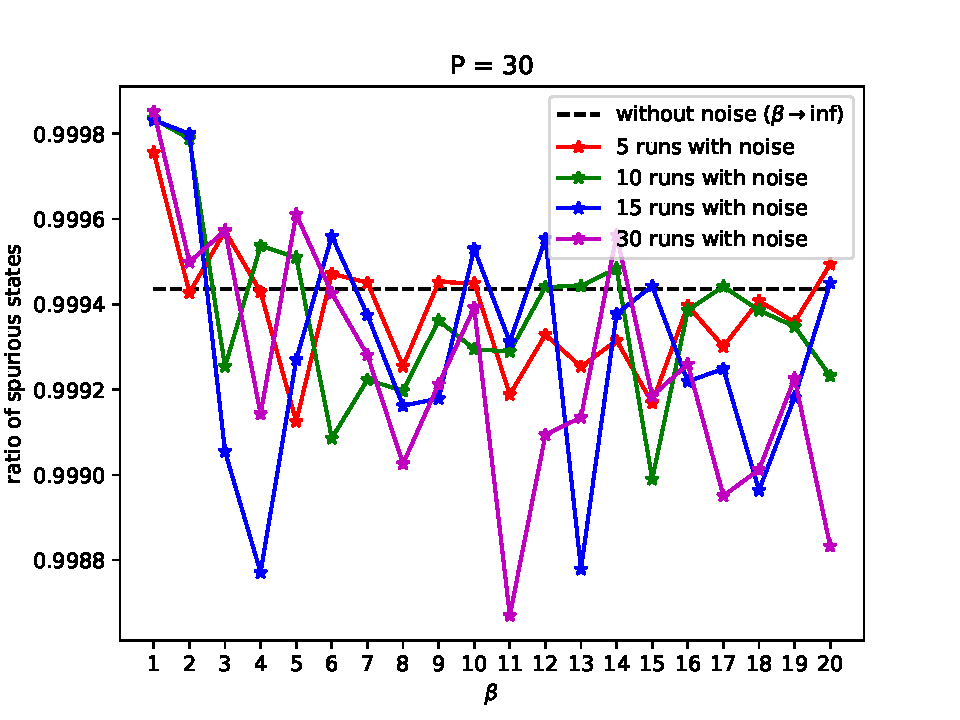
\includegraphics[width=0.63\textwidth]{../pics/fig_P30_w-noise.pdf}
    \caption{Zusammenhang zwischen der inversen Temperatur $\beta$ und dem Anteil der "`spurious states"' für verschiedene Anzahlen von Iterationen mit endlicher Temperatur zu Beginn; \textit{Oben:} $P = 10$, \textit{Mitte:} $P = 20$, \textit{Unten:} $P = 30$}
    \label{P10}
\end{figure}
%zwei Graphen nebeneinander:
%\begin{minipage}{0.45\textwidth}
%  	\includegraphics[width=0.99\textwidth]{A1_1__ValidationMat_Custom.eps} 
%\end{minipage}
%\begin{minipage}{0.45\textwidth}
%	\includegraphics[width=0.99\textwidth]{A1_1__ValidationMat_Builtin.eps}
%\end{minipage}

%\begin{figure}[ht]
%	\begin{minipage}{0.48\textwidth} 
%	\includegraphics[width=0.99\textwidth]{A1_1__ConvergingSteps.eps}
%  	\caption{Abbruchkriterium in Abh\"angigkeit der Iterationsschritte}
%	\end{minipage}
%	\hfill
%	\begin{minipage}{0.48\textwidth}
%	\includegraphics[width=0.99\textwidth]{A1_1__ConvergingEpsilon.eps}
%  	\caption{ben\"otigte Iterationsschrittzahl in Abh\"angigkeit des Abbruchkriteriums}
%	\end{minipage}
%\end{figure}


%\begin{figure}[h]
%  \centering
%  \includegraphics[width=0.6\textwidth]{A1_1__Runtime.eps}
%  \caption{Text}
%\end{figure}

\newpage
\begin{thebibliography}{}
\bibliographystyle{plain}
    \bibitem[1]{skript} U. Wolf und B. Bunk, "`CP II - Skript"', Humboldt-Universität zu Berlin, 2003
    \bibitem[2]{buch} J. Hertz, A. Krogh und R. Palmer, "`Introduction to the Theory of Neural Computation"',  Addison-Wesley, 1991
\end{thebibliography}
\end{document}


